\documentclass[UTF8,11pt]{ctexart}
\usepackage[a4paper,margin=22mm]{geometry}
\usepackage{graphicx,enumitem,amssymb,tabularx}
\usepackage[normalem]{ulem}
\usepackage{xeCJKfntef}
\setlength{\parindent}{0pt}
\setlength{\parskip}{.6em}
\sloppy
\begin{document}
\section*{2020年12月英语六级真题(第1套)}
\begin{center}
\includegraphics[width=.85\linewidth,height=.55\textheight,keepaspectratio]{2020-12-01.assets/figure-001-000.png}\end{center}

\subsection*{\textbf{Part I} \textbf{Writing} \textbf{( 30 minutes)}}


\textbf{Directions: }\textbf{\textit{For this part, you are allowed 30 minutes to write an essay on why students should be encouraged}} \textbf{\textit{to develop the ability to meet challenges. You should write at least 150 words but no more than 200 words.}}


\subsection*{\textbf{Part ll} \textbf{Li\&iening Comprehension} \textbf{( 30 minutes)}}


\subsection*{\textbf{Section A}}


\textbf{Directions: }\textbf{\textit{Jn this section, you will hear two long conversations. At the end of each conversation, you will}} \textbf{\textit{hear four questions. Both the conversation and the questions will be spoken only once. After you hear a}} \textbf{\textit{question, you must choose the best answer from the four choices marked A), B) }}, \textbf{C) }\textbf{\textit{and }}\textbf{D). }\textbf{\textit{Then mark}} \textbf{\textit{the corresponding letter on Answer Sheet 1 with a single line through the centre.}}


\textbf{Questions 1 to 4 are based on the conversation you have just heard.}


\textbf{1.}


\begin{itemize}[leftmargin=2em,itemsep=.2em,topsep=.4em]\item[A.] \textbf{She has not received any letter from the man.}
\item[B.] \textbf{Her claim has been completely disregarded;\textperiodcentered{}}
\item[C.] \textbf{She has failed 'to reach the manager again.}
\item[D.] \textbf{Her house has not been repaired in time.}
\end{itemize}

\textbf{2.}


\begin{itemize}[leftmargin=2em,itemsep=.2em,topsep=.4em]\item[A.] \textbf{Their caravan was washed away by the flood.}
\item[B.] \textbf{The ground floor of their cottage was flooded.}
\item[C.] \textbf{Their entire house was destroyed by the flood.}
\item[D.] \textbf{The roof of their cottage collapsed in the flood.}
\end{itemize}

\textbf{3.}


\begin{itemize}[leftmargin=2em,itemsep=.2em,topsep=.4em]\item[A.] \textbf{The woman's failure to pay her house insurance in time.}
\item[B.] \textbf{The woman's inaccurate description of the whole incident.}
\item[C.] \textbf{The woman's ignorance of the insurance company's policy.}
\item[D.] \textbf{The woman's misreading of the insurance company's letter.}
\end{itemize}

\textbf{4.}


\begin{itemize}[leftmargin=2em,itemsep=.2em,topsep=.4em]\item[A.] \textbf{Revise the terms and conditions of the contract.}
\item[B.] \textbf{Consult her lawyer about the insurance policy.}
\item[C.] \textbf{Talk to the manager of Safe House Insurance.}
\item[D.] \textbf{File a lawsuit against the insurance company.}
\end{itemize}

\textbf{Questions S to 8 are based on the conversation you have just heard.}


\textbf{5.}


\begin{itemize}[leftmargin=2em,itemsep=.2em,topsep=.4em]\item[A.] \textbf{They are both worried about the negative impact of technology.}
\item[B.] \textbf{They differ greatly in their knowledge of modem technology.}
\item[C.] \textbf{They disagree about the future of AI technology.}
\item[D.] \textbf{They work in different fields of AI technology.}
\end{itemize}

\textbf{6.}


\begin{itemize}[leftmargin=2em,itemsep=.2em,topsep=.4em]\item[A.] \textbf{Stimulating and motivating.}
\item[B.] \textbf{Simply writing Al software.}
\item[C.] \textbf{More demanding and requiring special training.}
\item[D.] \textbf{Less time-consuming and focusing on creation.}
\end{itemize}

\textbf{7.}


\begin{itemize}[leftmargin=2em,itemsep=.2em,topsep=.4em]\item[A.] \textbf{Old people would be taken care of solely by unfeeling robots.}
\item[B.] \textbf{Humans would be tired of communicating with one another.}
\item[C.] \textbf{Digital life could replace human civilization.}
\item[D.] \textbf{There could be jobs nobody wants to do.}
\end{itemize}

1\textbf{human beings.}


\textbf{8.}


\begin{itemize}[leftmargin=2em,itemsep=.2em,topsep=.4em]\item[A.] \textbf{It will be smarter than}
\item[B.] \textbf{Chips will be inserted in human brains.}
\item[C.] \textbf{It will take away humans' jobs altogether.}
\item[D.] \textbf{Life will become like a science fiction film.}
\end{itemize}

\subsection*{\textbf{Section B}}


\textbf{Directions: }\textbf{\textit{In this section, you will hear two passages. At the end of each passage, you will hear three or}} \textbf{\textit{four questions. Both the passage and the questions will be spoken only once }}\textbf{. }\textbf{\textit{After you hear a question }}\textbf{, }\textbf{\textit{you}} \textbf{\textit{must choose the best answer from the four choices marked A }}\textbf{) , }\textbf{\textit{B) }}\textbf{, C) }\textbf{\textit{and }}\textbf{D ). }\textbf{\textit{Then mark the}} \textbf{\textit{corresponding letter on Answer Sheet 1 with a single line through the centre.}}


\noindent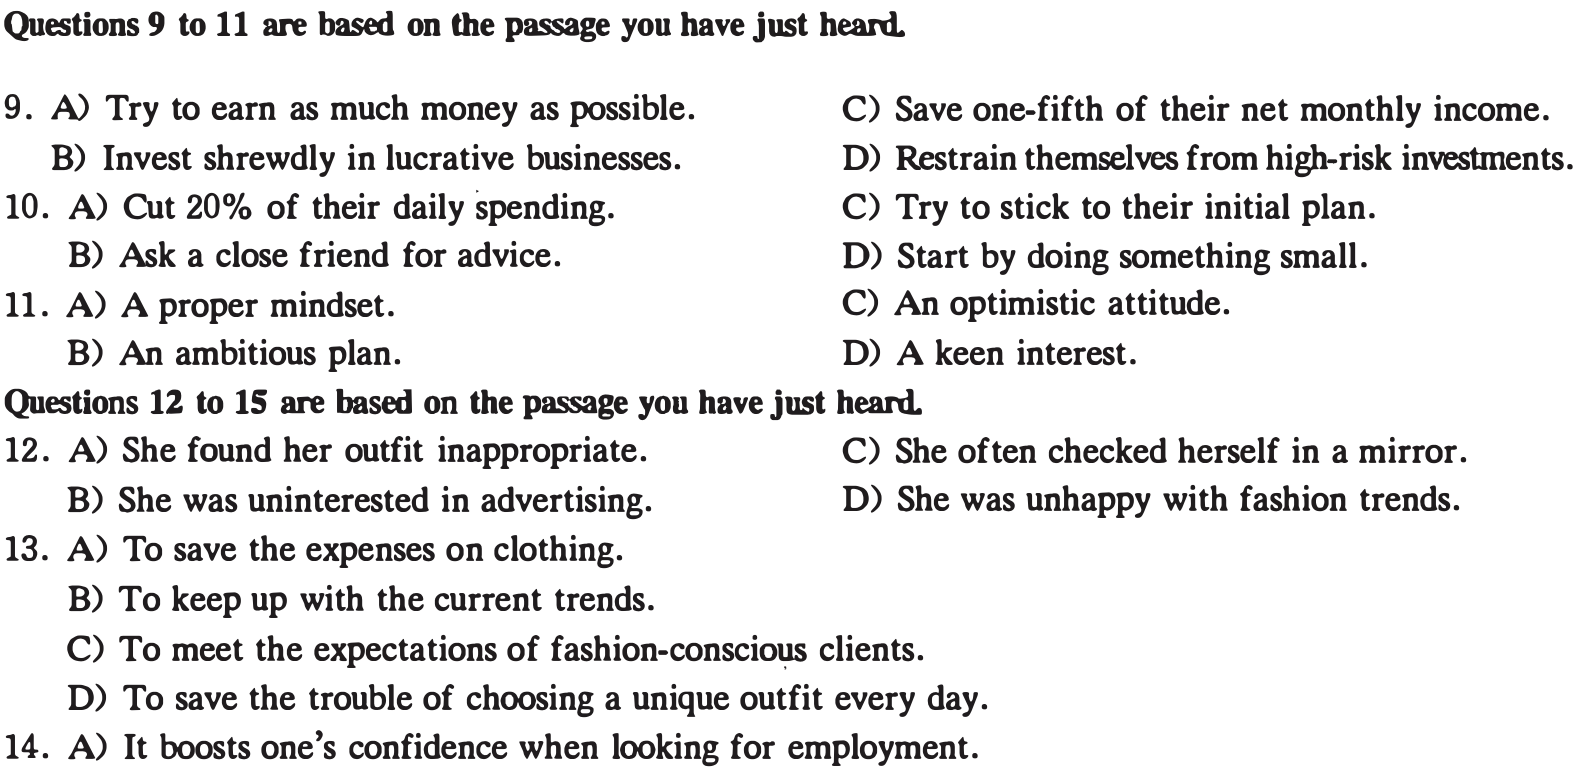
\includegraphics[width=\linewidth,height=.8\textheight,keepaspectratio]{2020-12-01.assets/char-002-line-002.png}\par

\begin{itemize}[leftmargin=2em,itemsep=.2em,topsep=.4em]\item[B.] \textbf{It matters a lot in jobs involving interaction with others.}
\item[C.] \textbf{It helps people succeed in whatever they are doing.}
\item[D.] \textbf{It enhances people's ability to work independently.}
\end{itemize}

\textbf{15.}


\begin{itemize}[leftmargin=2em,itemsep=.2em,topsep=.4em]\item[A.] \textbf{Design their own uniform to appear unique.}
\item[C.] \textbf{Do whatever is possible to look .smart.}
\end{itemize}

\textbf{•}


\begin{itemize}[leftmargin=2em,itemsep=.2em,topsep=.4em]\item[B.] \textbf{Fight the ever-changing trends in fashion.}
\item[D.] \textbf{Wear classic pieces to impress their clients.}
\end{itemize}

\subsection*{\textbf{Section C}}


\textbf{Directions: }\textbf{\textit{In this section, you will hear three recordings of lectures or talks followed by three or four}} \textbf{\textit{questions. The recordings will be played only once }}\textbf{. }\textbf{\textit{After you hear a question }}\textbf{, }\textbf{\textit{you must choose the best}} \textbf{\textit{answer from the four choices marked A), B), }}\textbf{C) }\textbf{\textit{and }}\textbf{D). }\textbf{\textit{Then mark the corresponding letter on Answer}} \textbf{\textit{Sheet 1 with a single line through the centre.}}


\textbf{Questions 16 to 18 are based on the recording you have just heard.}


\textbf{16.}


\begin{itemize}[leftmargin=2em,itemsep=.2em,topsep=.4em]\item[A.] \textbf{Their failure to accumulate wealth.}
\item[B.] \textbf{Their obsession with consumption.}
\item[C.] \textbf{The deterioration of the environment.}
\item[D.] \textbf{The ever-increasing costs of housing.}
\end{itemize}

\textbf{17.}


\begin{itemize}[leftmargin=2em,itemsep=.2em,topsep=.4em]\item[A.] \textbf{Things that we cherish most.}
\item[B.] \textbf{Things that boost efficiency.}
\item[C.] \textbf{Things that cost less money.}
\item[D.] \textbf{Things that are rare to find.}
\end{itemize}

\textbf{18.}


\begin{itemize}[leftmargin=2em,itemsep=.2em,topsep=.4em]\item[A.] \textbf{They are mostly durable.}
\item[B.] \textbf{They are easily disposable.}
\item[C.] \textbf{They serve multiple purposes.}
\item[D.] \textbf{They benefit the environment.}
\end{itemize}

\textbf{Questions 19 to 21 are based on the recording you have just heard.}


\textbf{19.}


\begin{itemize}[leftmargin=2em,itemsep=.2em,topsep=.4em]\item[A.] \textbf{All respondents were afraid of making a high expense claim.}
\item[B.] \textbf{A number of respondents gave an average answer of 400 miles.}
\item[C.] \textbf{Most of the respondents got compensated for driving 384 miles.}
\item[D.] \textbf{Over 10\% of the respondents lied about the distance they drove.}
\end{itemize}

\textbf{20.}


\begin{itemize}[leftmargin=2em,itemsep=.2em,topsep=.4em]\item[A.] \textbf{They endeavored to actually be honest.}
\item[B.] \textbf{They wanted to protect their reputation.}
\item[C.] \textbf{They cared about other people's claims.}
\item[D.] \textbf{They responded to colleagues' suspicion.}
\end{itemize}

\noindent\begin{tabularx}{\linewidth}{@{}lXXXX@{}}\textbf{21.} & \textbf{A.} \textbf{They seem positive.} & \textbf{B.} \textbf{They are illustrative.} & \textbf{C.} \textbf{They seem intuitive.} & \textbf{D.} \textbf{They are conclusive.}\\\end{tabularx}\par

\textbf{Questions 22 to 25 are based on the recording you have just heard.}


\textbf{22.}


\begin{itemize}[leftmargin=2em,itemsep=.2em,topsep=.4em]\item[A.] \textbf{Older people's aversion to new music.}
\item[B.] \textbf{Older people's changing musical tastes.}
\item[C.] \textbf{Insights into the features of good music.}
\item[D.] \textbf{Deterioration in the quality of new music.}
\end{itemize}

\textbf{23.}


\begin{itemize}[leftmargin=2em,itemsep=.2em,topsep=.4em]\item[A.] \textbf{They seldom listen to songs released in their teens.}
\item[B.] \textbf{They can make subtle distinctions about music.}
\item[C.] \textbf{They find all music sounds the same.}
\item[D.] \textbf{They no longer listen to new music.}
\end{itemize}

\textbf{24.}


\begin{itemize}[leftmargin=2em,itemsep=.2em,topsep=.4em]\item[A.] \textbf{The more you experience something, the better you'll appreciate it.}
\item[B.] \textbf{The more you experience something, the longer you'll remember it.}
\item[C.] \textbf{The more you are exposed to something, the deeper you'll understand it.}
\item[D.] \textbf{The more you'are exposed to something, the more familiar it'll be to you.}
\end{itemize}

\textbf{25.}


\begin{itemize}[leftmargin=2em,itemsep=.2em,topsep=.4em]\item[A.] \textbf{Teenagers are much more sensitive.}
\item[B.] \textbf{Teenagers are much more sentimental.}
\item[C.] \textbf{Teenagers' memories are more lasting.}
\item[D.] \textbf{Teenagers' emotions are more intense.}
\end{itemize}

\textbf{Part][} \textbf{Reading Comprehension} \textbf{( 40 minutes)}


\subsection*{\textbf{Section A}}


\noindent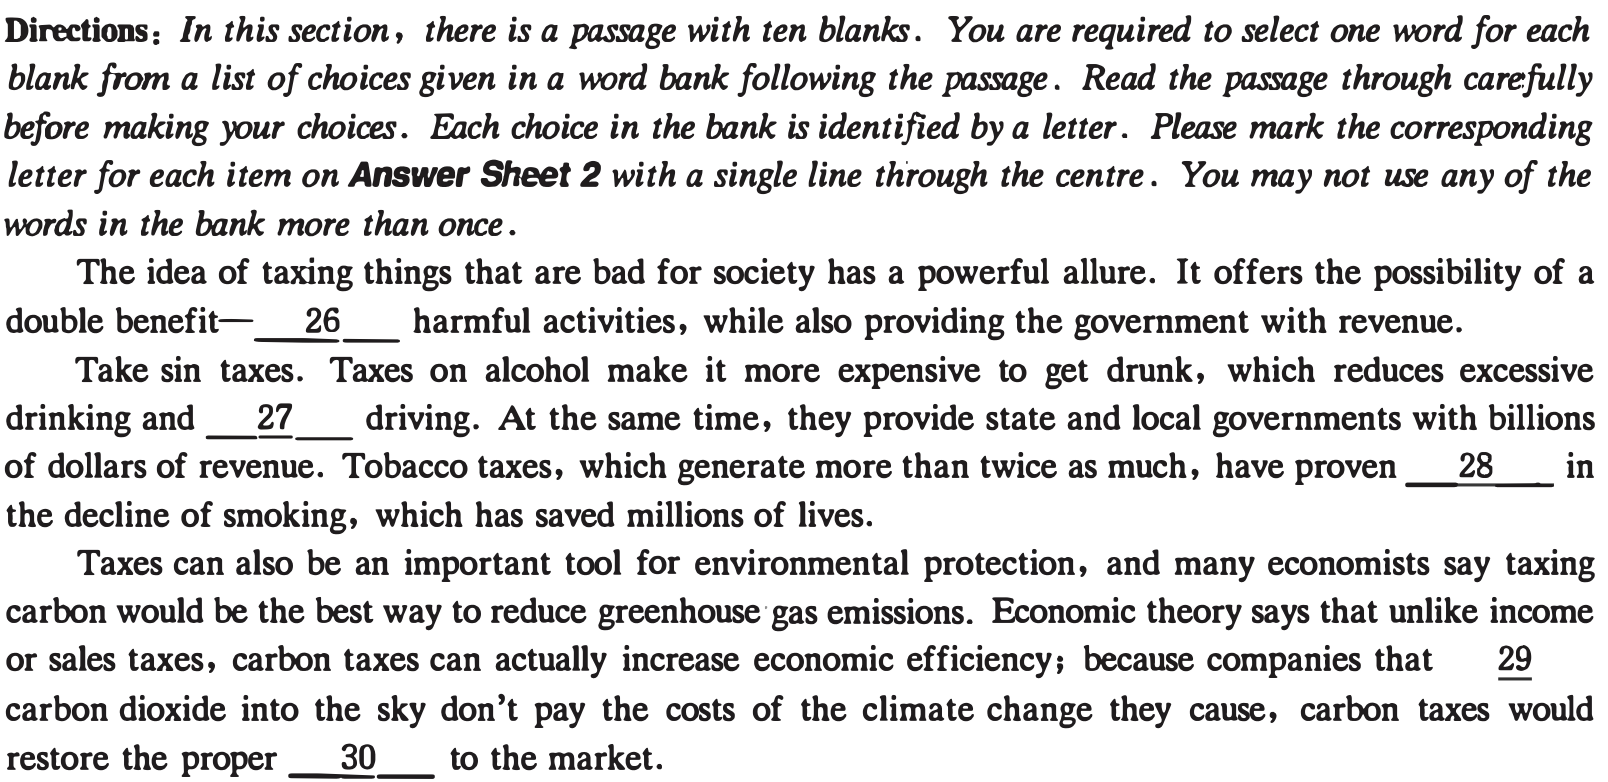
\includegraphics[width=\linewidth,height=.8\textheight,keepaspectratio]{2020-12-01.assets/char-003-line-011.png}\par

\textbf{In reality, carbon taxes alone won't be enough to halt global warming, but they would be a useful part} \textbf{of any climate plan. What's more, the revenue from this tax, which would \_fil\_ be hundreds of} \textbf{billions of dollars per year, could be handed out to citizens as a }\textbf{\uline{\_32\_}}\textbf{ or used to fund green} \textbf{infrastructure projects.}


\textbf{Similarly, a wealth tax has been put forward as a way to reduce inequality while raising revenue. The} \textbf{revenue from this tax, which some experts} \textbf{\uline{33}} \textbf{will be over \$ 4 trillion per decade, would be} \textbf{designated for housing, child care, health care and other government benefits. If you believe, as many} \textbf{do, that wealth inequality is} \textbf{\uline{34}} \textbf{bad, then these taxes improve society while also }\textbf{\uline{\_35\_}} \textbf{government }\textbf{\textit{coffers }}\textbf{( ½ .4).}


\begin{itemize}[leftmargin=2em,itemsep=.2em,topsep=.4em]\item[A.] \textbf{discouraging}
\item[B.] \textbf{dividend}
\item[C.] \textbf{emotional}
\item[D.] \textbf{fragments}
\item[E.] \textbf{impaired}
\item[F.] \textbf{imprisoned}
\item[G.] \textbf{incentives}
\item[H.] \textbf{inherently}
\item[I.] \textbf{initially}
\item[J.] \textbf{instrumental} \textbf{0) swelling}
\item[K.] \textbf{merging}
\item[L.] \textbf{predict}
\item[M.] \textbf{probably}
\item[N.] \textbf{pump}
\end{itemize}

\subsection*{\textbf{Section B}}


\textbf{Directions: }\textbf{\textit{In this section, you are going to read a passage with ten statements attached to it. F.ach}} \textbf{\textit{statement contains information given in one of the paragraphs. Identify the paragraph from which the}} \textbf{\textit{information is derived. You may choose a paragraph more than once. F.ach paragraph is marked with a}} \textbf{\textit{letter. Answer the questions by marking the corresponding letter on Answer Sheet 2.}} \textbf{The Challenges for Artificial Intelligence in Agriculture}


\noindent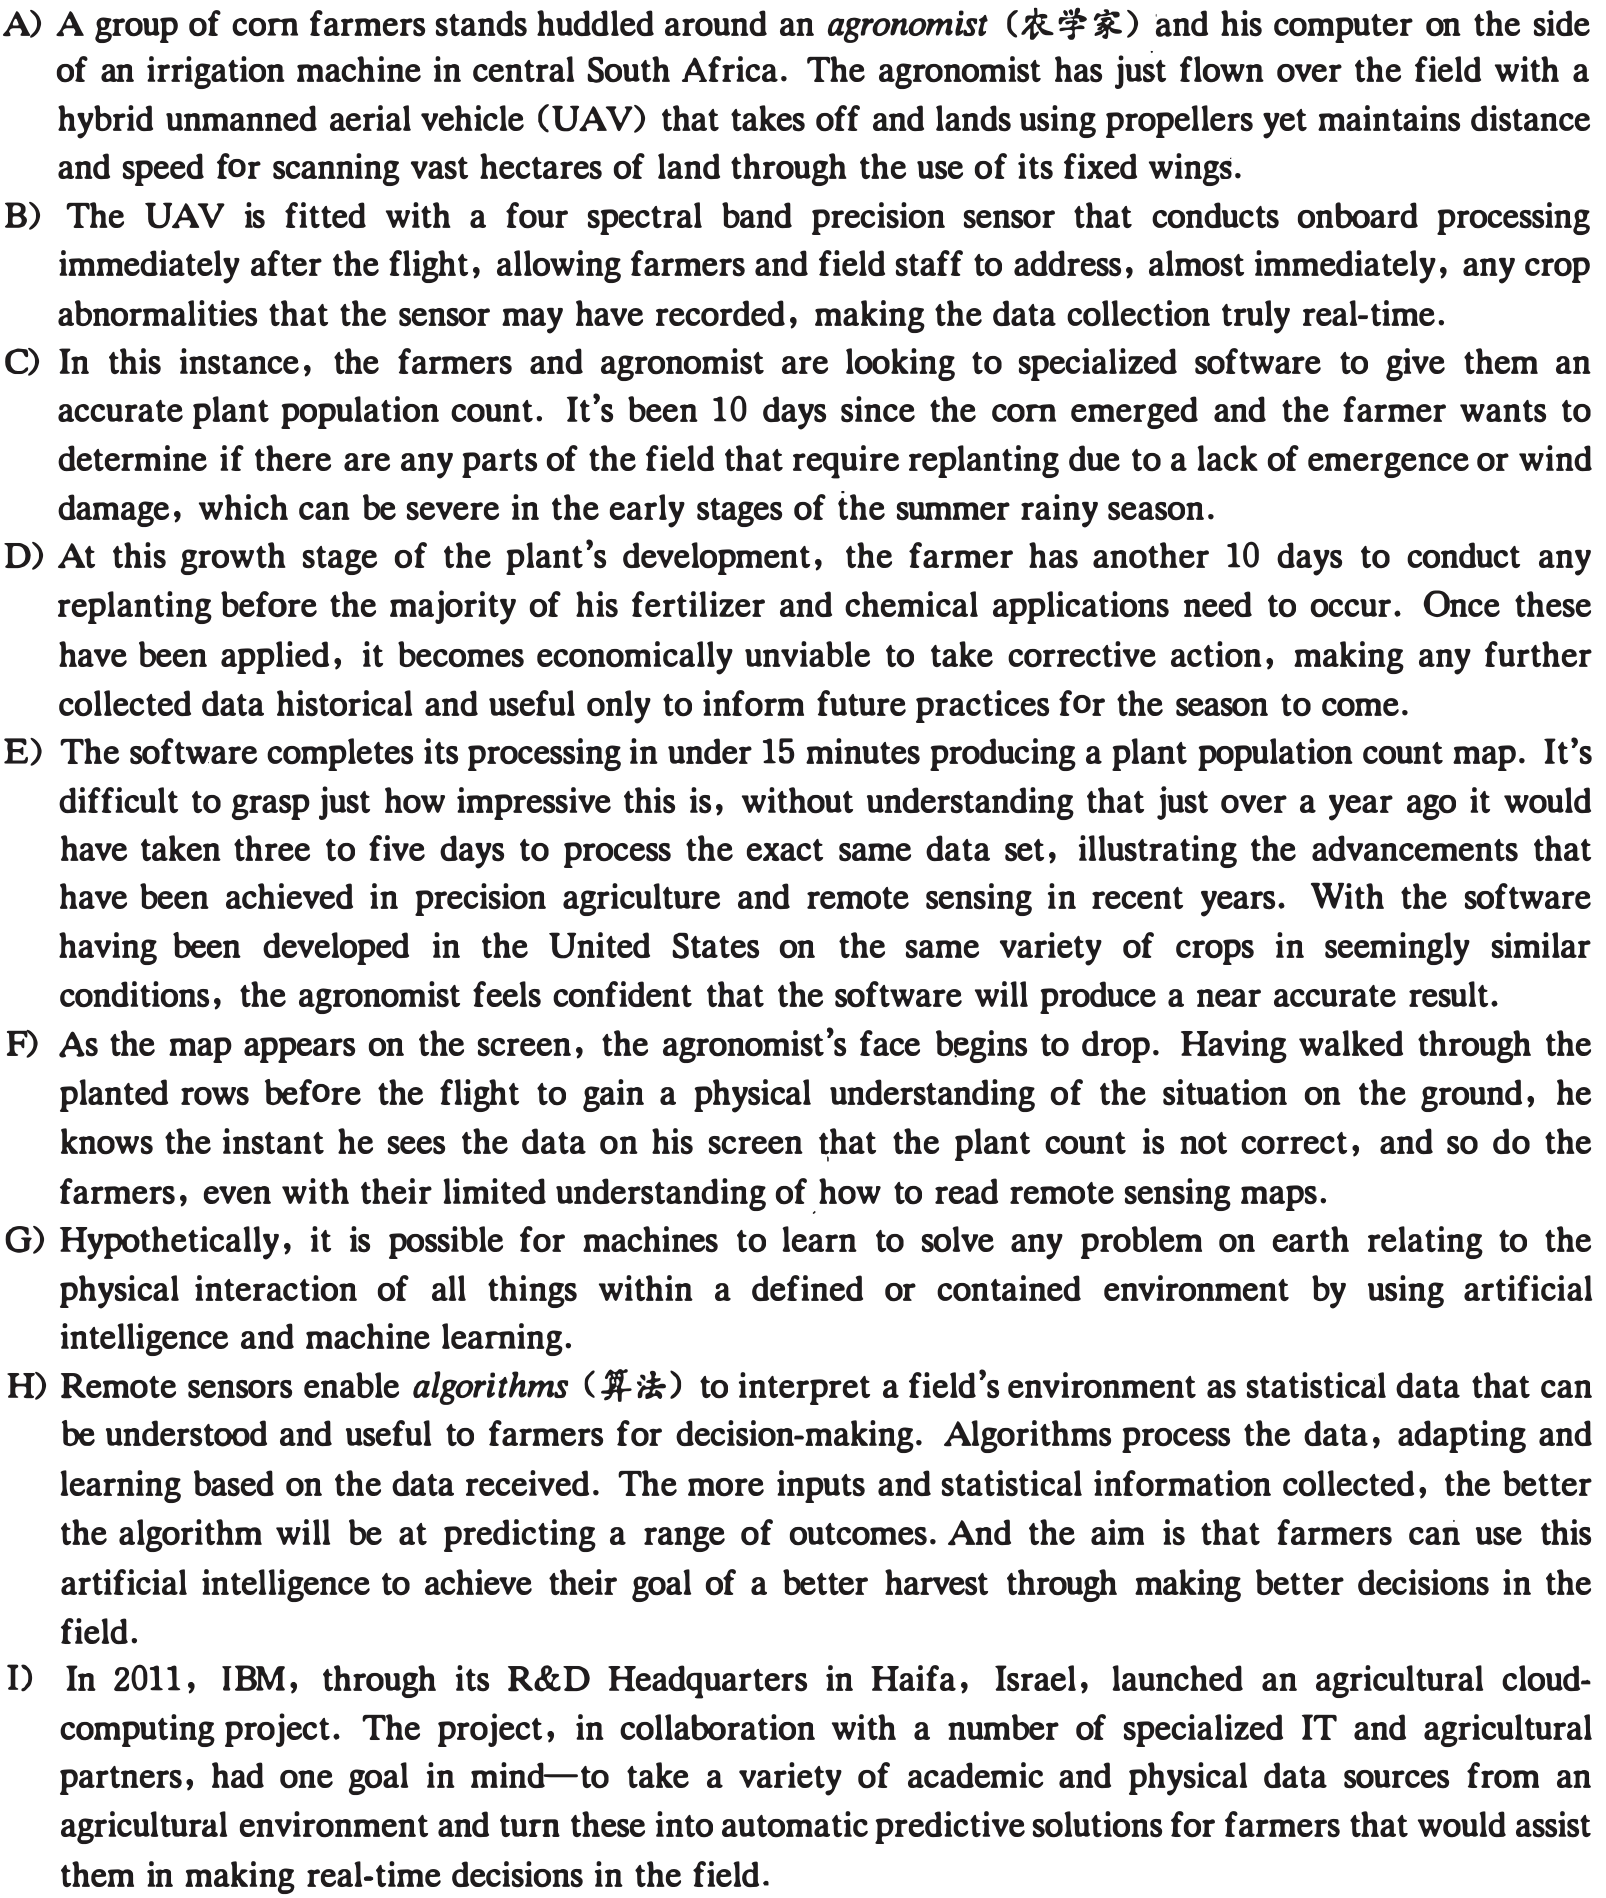
\includegraphics[width=\linewidth,height=.8\textheight,keepaspectratio]{2020-12-01.assets/char-004-line-002.png}\par

J) \textbf{Interviews with some of the IBM project team members at the time revealed that the team believed it} \textbf{was entirely possible to "algorithm" agriculture, meaning that algorithms could solve any problem in}


\noindent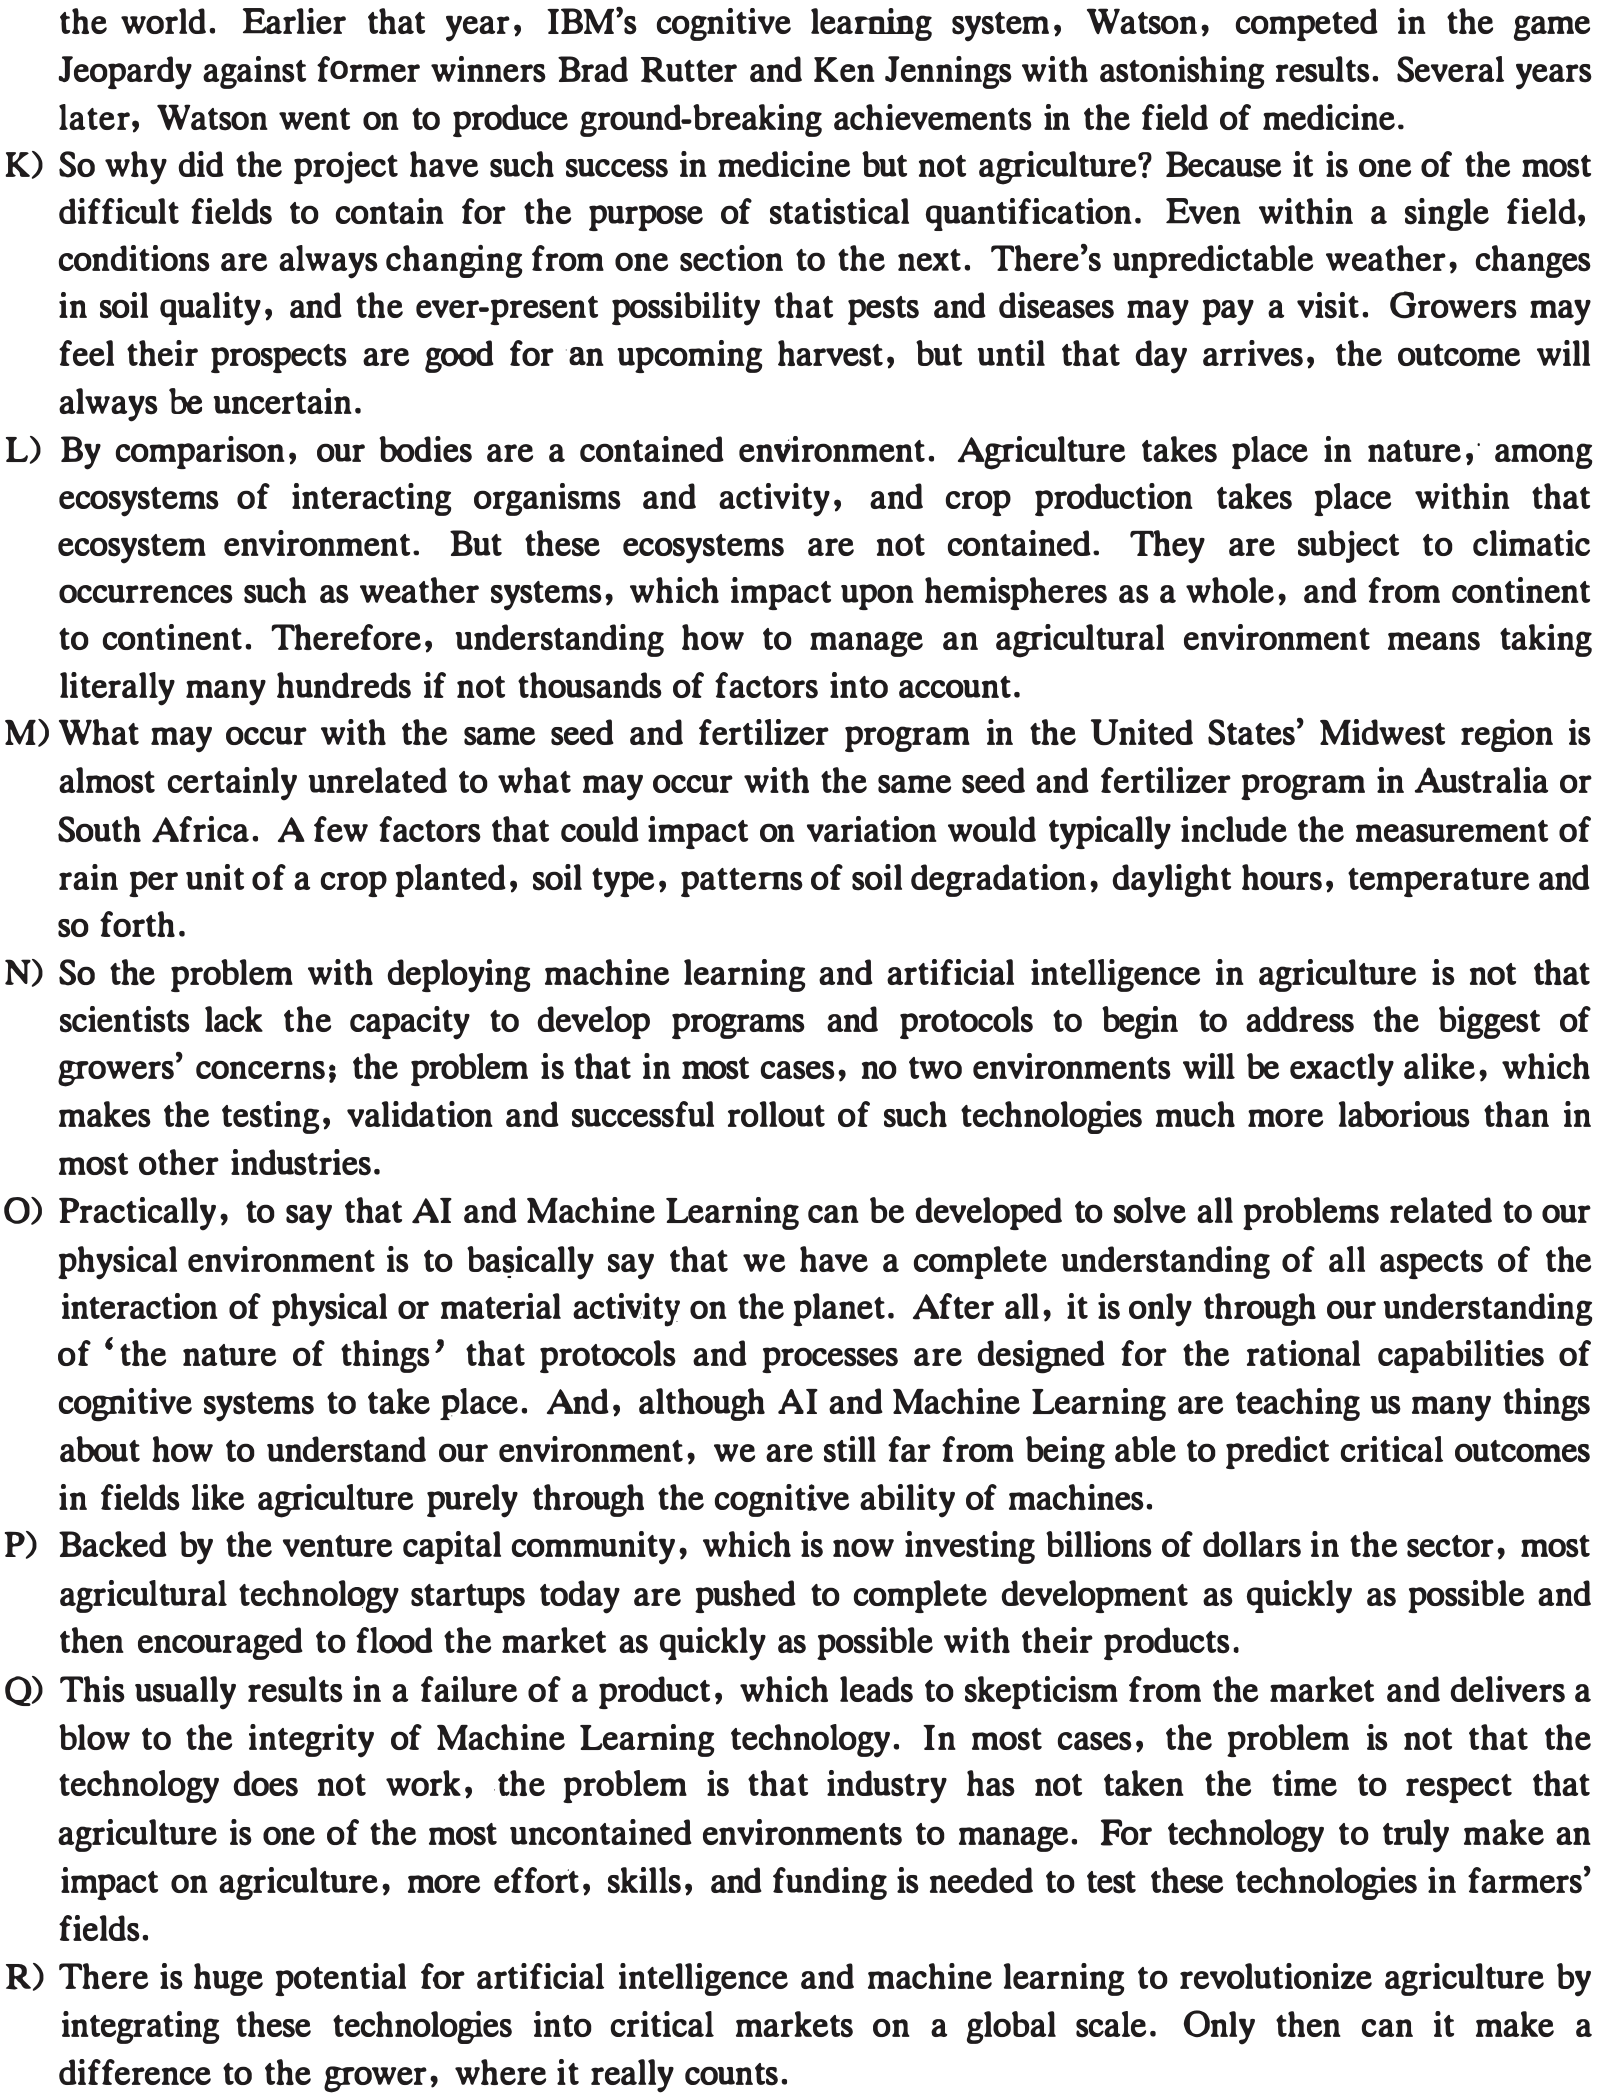
\includegraphics[width=\linewidth,height=.8\textheight,keepaspectratio]{2020-12-01.assets/char-005-line-000.png}\par

\textbf{36. Farmers will not profit from replanting once they have \textperiodcentered{}applied most of the \textperiodcentered{} fertilizer and other}


\textbf{chemicals to their fields.}


\textbf{37. Agriculture differs from the medical science of the human body in that its environment is not a}


\textbf{contained one.}


\noindent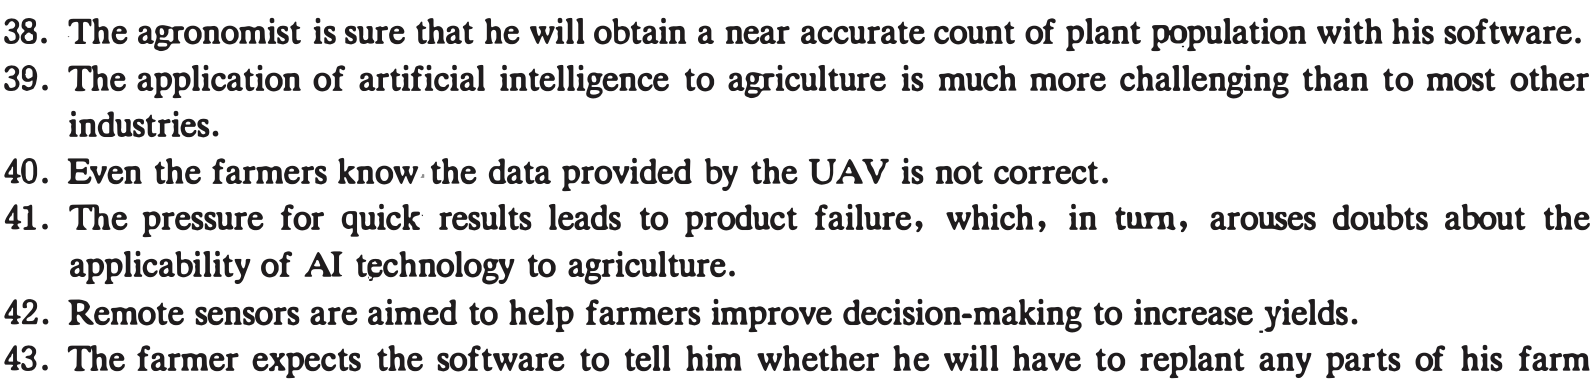
\includegraphics[width=\linewidth,height=.8\textheight,keepaspectratio]{2020-12-01.assets/char-006-line-000.png}\par

\textbf{fields.}


\textbf{44 .. Agriculture proves very difficult to quantify because of the constantly changing conditions involved.}


\textbf{45. The same seed and fertilizer program may yield completely different outcomes in different places.}


\noindent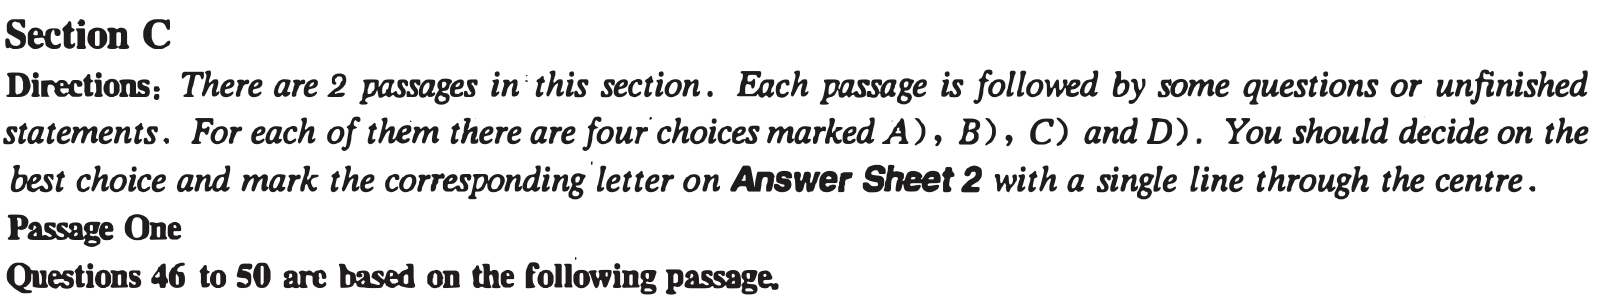
\includegraphics[width=\linewidth,height=.8\textheight,keepaspectratio]{2020-12-01.assets/char-006-line-004.png}\par

\textbf{What is the place of art in a culture of inattention? Recent visitors to the Louvre report that tourists} \textbf{can now spend only a minute in front of the Mona Lisa before being asked to move on. Much of that time,} \textbf{for some of them, is spent taking photographs not even of the painting but of themselves with the painting} \textbf{in the background.}


\textbf{One view is that we have democratised' tourism and gallery-going so much that we have made it} \textbf{effectively impossible to appreciate what we've travelled to see. In this oversubscribed society, experience} \textbf{becomes a commodity like any other. There are queues to climb Mt. Jolmo Lungma as well as to see} \textbf{famous paintings. Leisure, thus conceived, is hard labour, and returning to work becomes a well-eameq} \textbf{break from the ordeal.}


\noindent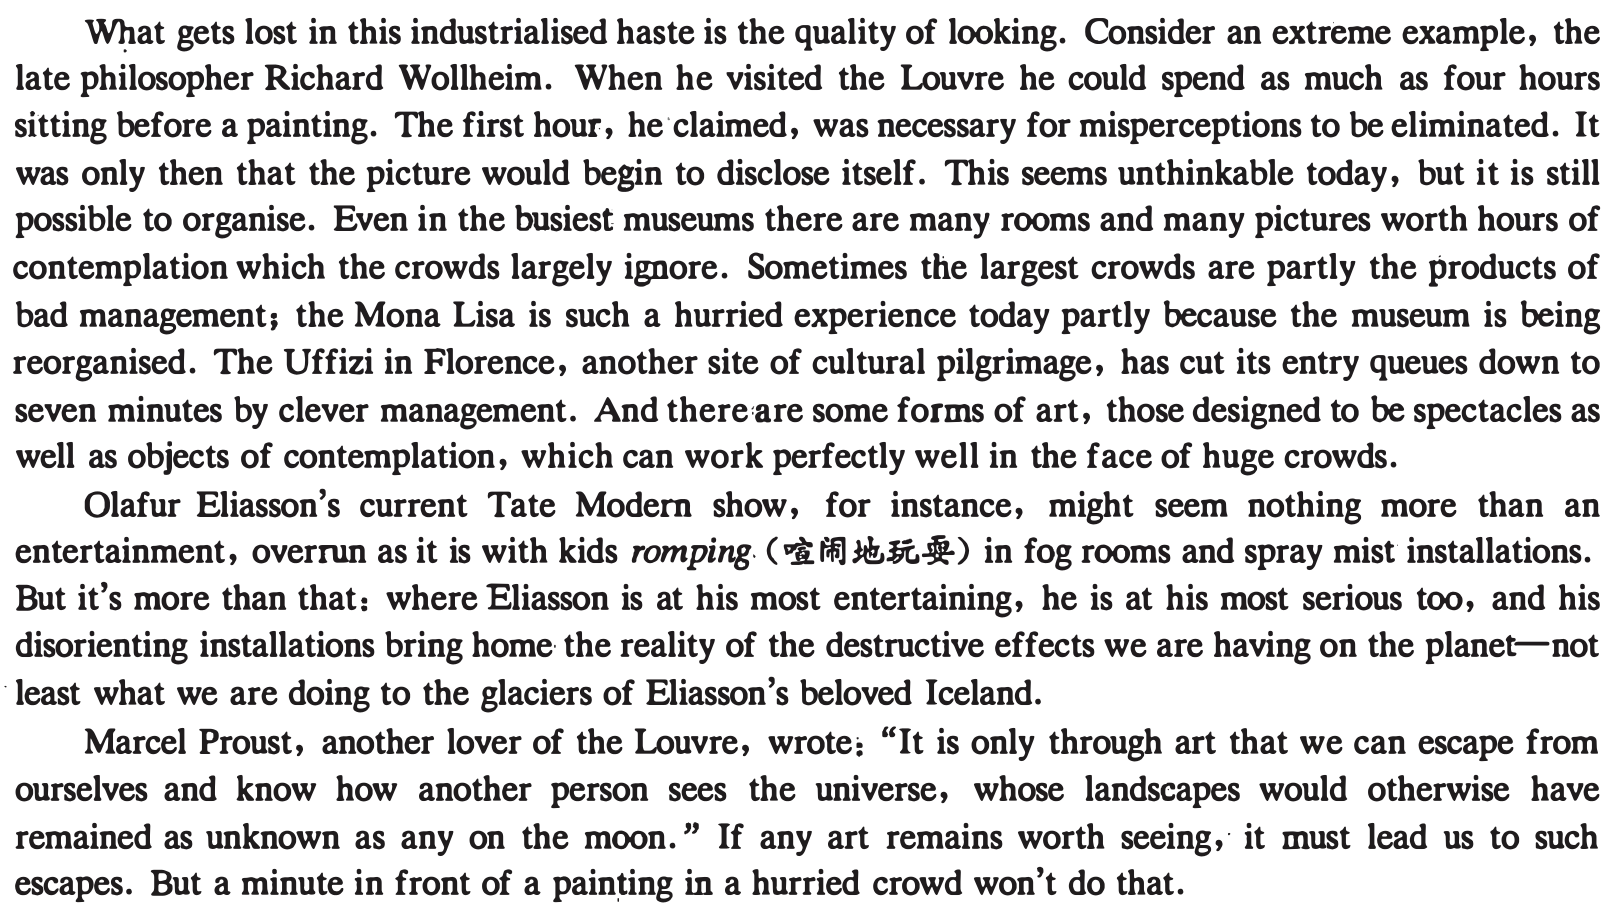
\includegraphics[width=\linewidth,height=.8\textheight,keepaspectratio]{2020-12-01.assets/char-006-line-007.png}\par

\textbf{46. What does the scene at the Louvre demonstrate according to the author?}


\begin{itemize}[leftmargin=2em,itemsep=.2em,topsep=.4em]\item[A.] \textbf{The enormous appeal of a great piece of artistic work to tourists.}
\item[B.] \textbf{The near impossibility of appreciating art in an age of mass tourism.}
\end{itemize}

\begin{itemize}[leftmargin=2em,itemsep=.2em,topsep=.4em]\item[C.] \textbf{The ever-growing commercial value of long-cherished artistic works.}
\item[D.] \textbf{The real difficulty in getting a glimpse at a masterpiece. amid a crowd.}
\end{itemize}

\textbf{4 7. Why did the late philosopher Richard Wollheim spend four hours before a picture?}


\begin{itemize}[leftmargin=2em,itemsep=.2em,topsep=.4em]\item[A.] \textbf{It takes time to appreciate a piece o\_f art fully.}
\item[B.] \textbf{It is quite common to misinterpret artistic works.}
\item[C.] \textbf{The longer people contemplate a picture, the more likely they will enjoy it.}
\item[D.] \textbf{The more time one spends before a painting, the more valuable one finds it.}
\end{itemize}

\textbf{48. What does the case of the Uffizi in Florence show?}


\begin{itemize}[leftmargin=2em,itemsep=.2em,topsep=.4em]\item[A.] \textbf{Art works in museums should be better taken care of.}
\item[B.] \textbf{Sites of cultural pilgrimage are always flooded with visitors.}
\item[C.] \textbf{Good management is key to handling large crowds of visitors.}
\item[D.] \textbf{Large crowds of visitors cause management problems for museums.}
\end{itemize}

\textbf{49. What do we learn from Olafur Eliasson's current Tate Modern show?}


\begin{itemize}[leftmargin=2em,itemsep=.2em,topsep=.4em]\item[A.] \textbf{Children learn to appreciate art works most effectively while they are playing.}
\item[B.] \textbf{It is possible to combine entertainment with appreciation of serious art.}
\item[C.] \textbf{Art works about the environment appeal most to young children.}
\item[D.] \textbf{Some forms of art can accommodate huge crowds of visitors.}
\end{itemize}

\textbf{50. What can art do according to Marcel Proust?}


\begin{itemize}[leftmargin=2em,itemsep=.2em,topsep=.4em]\item[A.] \textbf{Enable us to live a much fuller life.}
\item[B.] \textbf{Allow us to escape the harsh reality.}
\item[C.] \textbf{Help us to see the world from a different perspective.}
\item[D.] \textbf{Urge us to explore the unknown domain of the universe.}
\end{itemize}

\subsection*{\textbf{Passage Two}}


\textbf{Questions 51 to SS are based on the following passage.}


\textbf{Every five years, the government tries to tell Americans what to put in their bellies. Eat more} \textbf{vegetables. Dial back the fats. It's all based on the best available science for leading a healthy life. But the} \textbf{best available science also has a lot to say about what those food choices do to the environment, and some} \textbf{researchers are annoyed that new dietary recommendations of the USDA ( United States Department of} \textbf{Agriculture) released yesterday seem to utterly ignore that fact.} \textbf{Broadly, the 2016- 2020 dietary recommendations aim for balance: More vegetables, leaner meats} \textbf{and far less sugar.} \textbf{But Americans consume more calories per capita than almost any other country in the- world. So the} \textbf{things Americans eat have a huge impact on climate change. Soil tilling releases carbon dioxide, and} \textbf{delivery vehicles emit exhaust. The government's dietary guidelines could have done a lot to lower that} \textbf{climate cost. Not just because of their position of authority: The guidelines drive billions of dollars of food} \textbf{production through federal programs like school lunches and nutrition assistance for the needy.} \textbf{On its own, plant and animal agriculture contributes 9 percent of all the country's greenhouse gas} \textbf{emissions. That's not counting the fuel burned in transportation, processing, refrigeration, and other} \textbf{waypoints between farm and belly. Red meats are among the biggest and most notorious emitters, but} \textbf{trucking a salad from California to Minnesota in January also carries a significant burden. And greenhouse} \textbf{gas emissions aren't the whole story. Food production is the largest user of fresh water, largest contributor} \textbf{to the loss of biodiversity, and a major contributor to using up natural resources.} \textbf{All of these points and more showed up in the Dietary Guidelines Advisory Committee's scientific} \textbf{report, released last February. Miriam Nelson chaired the subcommittee in charge of sustainability for the} \textbf{report, and is disappointed that eating less meat and buying local food aren't in the final product.} \textbf{"Especially if you consider that eating less meat, especially red and processed, has health benefits," she} \textbf{says.}


\textbf{So what happened? The official response is that sustainability falls too far outside the guidelines'} \textbf{official scope, which is to provide "nutritional and dietary information."} \textbf{Possibly the agencies in charge of drafting the decisions are too close to the industries they are} \textbf{supposed to regulate. On one hand, the USDA is compiling dietary advice. On the other, their clients are} \textbf{US agriculture companies.} \textbf{The line about keeping the guidelines' scope to nutrition and diet doesn't ring quite right with} \textbf{researchers. David Wallinga, for example, says, "In previous guidelines, they've always been concerned} \textbf{with things like food security-which is presumably the mission of the USDA. You absolutely need to be} \textbf{worried about climate impacts and future sustainability if you want secure food in the future."}


\textbf{51. Why are some researchers irritated at the USDA's 2016 - 2020 Dietary Guidelines?}


\begin{itemize}[leftmargin=2em,itemsep=.2em,topsep=.4em]\item[A.] \textbf{It ignores the harmful effect of red meat and processed food on health.}
\item[B.] \textbf{Too much emphasis is given to-eating less meat and buying local food.}
\item[C.] \textbf{The dietary recommendations are not based on medical science.}
\item[D.] \textbf{It takes no notice of the potential impact on the environment.}
\end{itemize}

\textbf{52. Why does the author say the USDA could \textperiodcentered{}have contributed a lot to lowering the climate cost through}


\textbf{its dietary guidelines?}


\begin{itemize}[leftmargin=2em,itemsep=.2em,topsep=.4em]\item[A.] \textbf{It has the capacity and the financial resources to do so.}
\item[B.] \textbf{Its researchers have already submitted relevant proposals.}
\item[C.] \textbf{Its agencies in charge of drafting the guidelines have the expertise.}
\item[D.] \textbf{It can raise students' environmental awareness through its programs.}
\end{itemize}

\textbf{53. What do we learn from the Dietary Guidelines Advisory Committee's scientific report?}


\begin{itemize}[leftmargin=2em,itemsep=.2em,topsep=.4em]\item[A.] \textbf{Food is easily contaminated from farm to belly.}
\item[B.] \textbf{Greenhouse effect is an issue still under debate.}
\item[C.] \textbf{Modern agriculture has increased food diversity.}
\end{itemize}

\textbf{DLFarming consumes most of our natural resources.}


\textbf{54. What may account for the neglect of sustainability in the USDA's Dietary Guidelines according to the}


\textbf{author?}


\begin{itemize}[leftmargin=2em,itemsep=.2em,topsep=.4em]\item[A.] \textbf{Its exclusive concern with Americans' food safety.}
\item[B.] \textbf{Its sole responsibility for providing dietary advice.}
\item[C.] \textbf{Its close ties with the agriculture companies.}
\item[D.] \textbf{Its alleged failure to regulate the industries.}
\end{itemize}

\textbf{55. What should the USDA do to achieve food security according to David Wallinga?}


\begin{itemize}[leftmargin=2em,itemsep=.2em,topsep=.4em]\item[A.] \textbf{Give top priority to things like nutrition and food security.}
\item[B.] \textbf{.Endeavor to ensure the sustainable development of agriculture.}
\item[C.] \textbf{Fulfill its mission by closely cooperating with the industries.}
\item[D.] \textbf{Study the long-term impact of climate change on food production.}
\end{itemize}

\subsection*{\textbf{Part N} \textbf{Translation} \textbf{( 30 minutes)}}


\textbf{Directions: }\textbf{\textit{For this part }}, \textbf{\textit{you are allowed 30 minutes to translate a passage from Chinese into English }}. • \textbf{\textit{You}} \textbf{\textit{should write your answier on Answer Sheet 2.}}


北京大兴国际机场位于天安门广场以南46公里处,于2019年9月30日投入使用。该巨型工程于2014 年开工建设,高峰时工地上有4万多工人。航站楼设计紧凑,可以允许最大数量的飞机直接停靠在最靠近航站楼中心的位置,这给乘客提供了极大的方便。航站楼共有82个登机口,但乘客通过安检后,只需不到8分钟就能抵达任何一个登机口。机场的设计可确保每小时300架次起降。机场年客运量2040年将达到1亿人次，有望成为世界上最繁忙的机场。

\end{document}